\documentclass[journal]{IEEEtran}
\IEEEoverridecommandlockouts
\usepackage{cite}
\usepackage{amsmath,amssymb,amsfonts}
\usepackage{graphicx}
\usepackage{booktabs}
\usepackage{multirow}
\usepackage{array}
\usepackage{xcolor}
\usepackage{algorithm}
\usepackage{algpseudocode}
\usepackage{tikz}
\usetikzlibrary{positioning,arrows.meta,shapes.geometric,fit,calc}
\usepackage[hidelinks]{hyperref}
\renewcommand{\algorithmicrequire}{\textbf{Input:}}
\renewcommand{\algorithmicensure}{\textbf{Output:}}

\begin{document}


\renewcommand{\thetable}{S\arabic{table}}
\renewcommand{\thefigure}{S\arabic{figure}}
\renewcommand{\thesection}{S\arabic{section}}
\title{Supplementary Material for ``Stagnation-Triggered Interventions for Wrapper Feature Selection: RL-DOHO and a Controlled Test of Learned Operator Selection''}
\author{Preetha~Evangeline~D, Prasenjit~Choudhury, Shreyansh~Dabgar, and Aditya~Jha}
\maketitle

This supplement gives the details of parts of the study that are summarized in the main text. Code, notebooks and per-run results are at \url{https://github.com/adj-04/rl-doho}.
\section{Sensitivity to the operator implementation}
An earlier version of this study used simplified three-phase versions of the DO and HO update rules, a dense start on all datasets, the old reward and a budget defined in iterations. Table~\ref{tab:sens} and Fig.~\ref{fig:sens} compare the two versions on the six datasets of the main study, with the same splits and seeds.
\begin{itemize}
\item \textbf{Simplified rules:} RL-DOHO was ahead of DO in 41 of the 60 runs and behind in 13. It was level with HO (30 against 29) and behind the GA (20 against 39).
\item \textbf{Published rules:} the corresponding figures are 54 against 3, 28 against 29 and 18 against 40.
\item \textbf{The conclusions about the DO--HO family and the GA are unchanged:} clearly better than DO, level with HO, behind the GA. With the published rules the gap to DO widens, partly because the published DO stalls on the clinical problem.
\item \textbf{The comparison with binary PSO and GWO reversed.} Under v1, RL-DOHO was behind both (25 against 34 and 22 against 38 runs); under v2 it was ahead (50 against 8 and 47 against 13). This change most likely comes from the sparse start, which RL-DOHO keeps and the two baselines drift away from.
\item \textbf{Gene data:} the new configuration reduced the subsets of the DO--HO family from about 2,100 genes to 99--157 and lowered their fitness substantially. Their mean test accuracy fell by 1.2--3.2 points, while that of the GA, BPSO and BGWO changed by about 0.2 points or less.
\item \textbf{GA, BPSO and BGWO} also improved in fitness under the sparse start.
\end{itemize}

\begin{table*}[t]
\centering
\caption{Sensitivity analysis: mean fitness and test accuracy (\%) of the wrapper methods under the earlier configuration (v1: simplified DO/HO rules, dense start, old reward) and the final one (v2), and mean number of selected genes on gene data. On the clinical data the GA, BPSO and BGWO runs are shared by both versions.}
\label{tab:sens}
\footnotesize
\setlength{\tabcolsep}{4pt}
\begin{tabular}{@{}lcccccccccc@{}}
\toprule
& \multicolumn{4}{c}{Rheumatic} & \multicolumn{4}{c}{Gene expression (5 datasets)} & \multicolumn{2}{c}{Genes selected} \\
\cmidrule(lr){2-5}\cmidrule(lr){6-9}\cmidrule(l){10-11}
Method & Fit.\ v1 & Fit.\ v2 & Acc.\ v1 & Acc.\ v2 & Fit.\ v1 & Fit.\ v2 & Acc.\ v1 & Acc.\ v2 & v1 & v2 \\
\midrule
RL-DOHO & 0.1845 & 0.1832 & 84.3 & 84.3 & 0.1396 & 0.0786 & 84.4 & 83.2 & 2098 & 157 \\
DO & 0.1871 & 0.2280 & 84.1 & 80.0 & 0.1443 & 0.1113 & 83.8 & 81.2 & 2114 & 124 \\
HO & 0.1880 & 0.1838 & 83.8 & 84.3 & 0.1382 & 0.0816 & 85.0 & 81.8 & 2110 & 99 \\
DOHO & 0.1882 & 0.1857 & 84.0 & 84.5 & 0.1403 & 0.0966 & 84.7 & 82.0 & 2114 & 115 \\
\midrule
GA & 0.1821 & (same) & 84.4 & (same) & 0.1432 & 0.0616 & 83.5 & 83.5 & 2006 & 121 \\
BPSO & 0.1828 & (same) & 84.5 & (same) & 0.1344 & 0.1192 & 83.8 & 83.6 & 2122 & 670 \\
BGWO & 0.1894 & (same) & 83.8 & (same) & 0.1362 & 0.1014 & 83.8 & 83.9 & 2031 & 772 \\
\bottomrule
\end{tabular}
\end{table*}

\begin{figure*}[t]
\centering
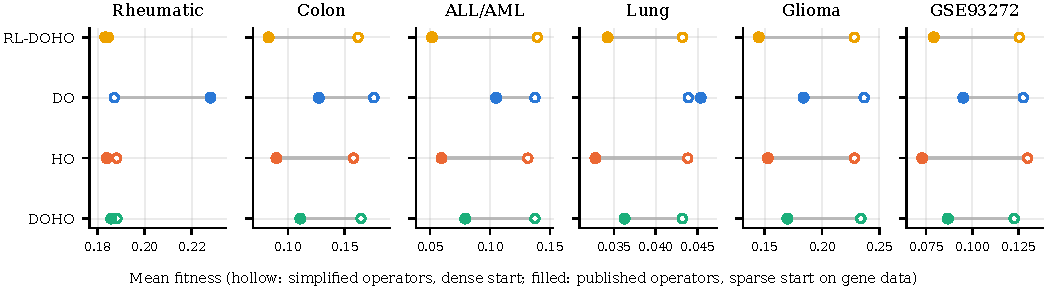
\includegraphics[width=\textwidth]{figs/sensitivity.pdf}
\caption{Mean fitness of the DO--HO family under the earlier configuration (hollow) and the final one (filled), per dataset.}
\label{fig:sens}
\end{figure*}


\section{Cost}
Every method received the same budget of fitness evaluations, but the budget also counts repeated subsets, and those are served from the cache. The real cost of a run is therefore set by the number of distinct subsets it evaluates (Table~\ref{tab:cost}).
\begin{itemize}
\item On the new clinical splits, RL-DOHO evaluated 83 distinct subsets per run, against 131 for HO, 132 for the GA and 245 for binary PSO. At about 3.6~s per new subset on the free Colab runtime we used, that is roughly 5, 8, 8 and 15 minutes per run from an empty cache.
\item On the tabular data the pattern was the same (381 against 596, 633 and 1,018 subsets).
\item Fewer distinct subsets also means less exploration. DO evaluated the fewest and was the weakest method, and binary GWO, which also evaluated few, ranked well on the tabular data but poorly on the clinical splits. The count is a cost advantage, not a quality signal.
\item The algorithms' own overhead was below 1.5~ms per evaluation for every method, even at $D=7{,}129$. That is negligible next to a fitness evaluation (about 20~ms for the tabular KNN and 3.6~s for the clinical models).
\item The per-evaluation cost on the clinical data was recorded on one split only, on one shared cloud runtime.
\end{itemize}

\begin{table}[h]
\centering
\caption{Cost: mean number of distinct subsets evaluated per run on the two new clinical splits (budget 252) and the tabular datasets (budget 1,020), and algorithm overhead in milliseconds per fitness evaluation on a near-free fitness function, by number of features $D$.}
\label{tab:cost}
\footnotesize
\setlength{\tabcolsep}{3pt}
\begin{tabular}{@{}lcccccc@{}}
\toprule
& \multicolumn{2}{c}{Distinct subsets} & \multicolumn{4}{c}{Overhead (ms/evaluation)} \\
\cmidrule(lr){2-3}\cmidrule(l){4-7}
Method & Clinical & Tabular & $D=14$ & 44 & 2,000 & 7,129 \\
\midrule
RL-DOHO & 83 & 381 & 0.08 & 0.06 & 0.26 & 0.77 \\
DO & 13 & 24 & 0.03 & 0.03 & 0.31 & 1.41 \\
HO & 131 & 596 & 0.06 & 0.06 & 0.12 & 0.26 \\
DOHO & 77 & 290 & 0.05 & 0.04 & 0.21 & 0.62 \\
\midrule
GA & 132 & 633 & 0.05 & 0.04 & 0.09 & 0.19 \\
BPSO & 245 & 1018 & 0.02 & 0.02 & 0.09 & 0.27 \\
BGWO & 54 & 237 & 0.08 & 0.08 & 0.20 & 0.48 \\
GA+SI & 171 & 771 & 0.08 & 0.07 & 0.12 & 0.24 \\
HO+SI & 140 & 656 & 0.07 & 0.07 & 0.14 & 0.27 \\
\bottomrule
\end{tabular}
\end{table}

\section{Controller extensions: protocol and the warm-start result}
The main text finds that a learned controller (UCB1 or tabular Q-learning) does no better than random choice of the intervention, and gives two likely causes: the controller gets few decisions per run, and the moves are complementary rather than ranked. We designed one experiment for each cause and one for the controller's information. All of them use the same code as the main study, and the protocol below was fixed before any of them was run. The notebook (Notebook 11 in the repository) runs it as specified.

\emph{The three extensions.}
\begin{itemize}
\item \textbf{Warm start (more decisions).} Before each evaluated run, two warm-up runs of 1,020 evaluations on the same training split (optimizer seeds 1000+$s$ and 2000+$s$) are chained, and the evaluated run starts from the controller statistics they produce, halved and capped at ten pulls per move. Only the controller's statistics carry over; no subsets, populations or tabu entries do. The warm-up evaluations are reported as extra cost.
\item \textbf{A move pool that differs in kind (more to learn).} Seven moves: flip 1--3 features of the best subset (the original PERTURB), flip 4 to $\min(20, D/2)$ features, remove 1--3 selected features, swap 1--2 selected features for unselected ones, restart, one DO iteration and one HO iteration.
\item \textbf{Context.} A disjoint LinUCB bandit (L. Li et al., WWW 2010; $\alpha=1$, ridge 1) sees the share of the budget used, how long the search has been stuck, population diversity, the size of the best subset and whether the last move improved it.
\end{itemize}

\emph{Design.} Nine variants are run at three times the standard budget (3,060 evaluations, population 20) on the ten KNN datasets with ten seeds: random choice, UCB1 and LinUCB on the original four moves; random choice, UCB1 and LinUCB on the seven moves; and warm-started UCB1 (four and seven moves) and warm-started LinUCB (seven moves). At this budget the controller makes about 80--170 decisions per run, against about 30 at the standard budget.

\emph{Verification.} With the original four moves, no warm start and UCB1 or random choice, the extended code reproduces the main study's runs exactly: the same subsets are evaluated in the same order and the same result is returned. We checked this on a synthetic fitness and on real data before fixing the protocol, so the four-move variants double as a check against the main study's three-times-budget runs.

\emph{Hypotheses.} Pooled two-sided sign tests on fitness over 100 paired runs, Holm-corrected over the four:
\begin{itemize}
\item \textbf{H10a:} warm-started UCB1 against random choice, four moves.
\item \textbf{H10b:} UCB1 against random choice, seven moves.
\item \textbf{H10c:} LinUCB against random choice, seven moves.
\item \textbf{H10d:} warm-started LinUCB against random choice, seven moves.
\end{itemize}

\emph{Success criterion.} The controller is judged to earn its place only if at least one of H10a--d favours the learner at Holm $p<0.05$ and that variant is not significantly worse than the current RL-DOHO. Two diagnostics accompany the tests. The first is a Kruskal--Wallis test of whether the moves' rewards under random choice differ. The second is the correlation between how often a learner picks each move and that move's mean reward. Together they show whether there is anything to learn and whether it was learned. All outcomes are reported whichever way they fall.

\emph{What was run.} Of the four, only H10a (the warm start) was run, because it addresses the cause the main study identifies first (too few decisions per run). It used three variants: random choice, cold-started UCB1 (the current RL-DOHO) and warm-started UCB1, all with the four original moves, on the ten KNN datasets with ten seeds. H10b--d were not run and are reported as not run; with a single test, no multiplicity correction applies.

\emph{Verification.} The two four-move baselines reproduced the main study's three-times-budget runs exactly (200 of 200 runs identical).

\emph{Result.} H10a was not supported. The warm-started bandit reached lower fitness than random choice in 46 runs and higher in 53 ($p=0.55$; tabular 26 against 23, gene 20 against 30). Against the cold-started bandit it was ahead in 39 and behind in 61 (unadjusted $p=0.035$, Holm $p=0.070$ over the two comparisons with the current method), so the success criterion was not met. Test accuracy did not differ (42 against 42, 16 ties). The warm-up runs raised the number of distinct subsets evaluated per run by about 70\%. Each run made about 80--115 decisions.

\emph{Diagnostics.} Under random choice the four moves' rewards differed on every dataset (Kruskal--Wallis $p<0.001$). The cold-started bandit's choice frequencies matched the ranking of the moves' mean rewards on all ten datasets (Spearman 1.0), as did the warm-started bandit's (mean 0.96). However, the move with the highest mean reward, DO (0.10--0.13), improved the best subset in at most 11\% of uses, whereas PERTURB and HO did so in up to 28\% and 22\%. The reward gaps were also small relative to UCB1's exploration bonus, so the bandit's choices stayed close to uniform (DO 32\%, PERTURB 25\%, HO 22\%, RESTART 20\%). The bandit learned its reward; the reward did not track improvement of the best subset closely enough for that learning to pay off.


\section{Repeated clinical splits}
The main text summarizes the comparison on two further train/test splits of the rheumatic data (H8). Table~\ref{tab:splits} gives the full results: mean fitness and test accuracy on each split, mean per-run ranks over the 15 paired runs, and RL-DOHO's wins, ties and losses against each method.

\begin{table*}[h]
\centering
\caption{Repeated clinical splits: mean fitness and test accuracy (\%) over seeds 0--4 on the original split and two new splits, mean per-run rank over the 15 runs (1 = best of 13), and W/T/L of RL-DOHO against each method on fitness. Best value per column in bold.}
\label{tab:splits}
\footnotesize
\setlength{\tabcolsep}{4pt}
\begin{tabular}{@{}lccccccccc@{}}
\toprule
& \multicolumn{3}{c}{Fitness} & \multicolumn{3}{c}{Test accuracy} & \multicolumn{2}{c}{Rank} & \\
\cmidrule(lr){2-4}\cmidrule(lr){5-7}\cmidrule(lr){8-9}
Method & Original & Split 1 & Split 2 & Original & Split 1 & Split 2 & Fitness & Test acc. & W/T/L \\
\midrule
\textbf{RL-DOHO} & 0.1837 & 0.1852 & 0.1820 & 84.50 & \textbf{84.68} & 83.08 & 6.57 & 5.67 & -- \\
DO & 0.2368 & 0.2303 & 0.2325 & 79.12 & 79.37 & 78.15 & 12.93 & 12.93 & 15/0/0 \\
HO & 0.1843 & 0.1851 & \textbf{0.1785} & 84.32 & 84.63 & 82.97 & 4.50 & 7.50 & 5/1/9 \\
DOHO & 0.1856 & 0.1865 & 0.1804 & 84.46 & 84.64 & 83.04 & 8.27 & 6.73 & 8/2/5 \\
\midrule
GA & \textbf{0.1821} & \textbf{0.1849} & 0.1794 & 84.41 & 84.68 & 83.12 & \textbf{3.80} & 5.20 & 3/0/12 \\
BPSO & 0.1831 & 0.1854 & 0.1794 & 84.60 & 84.51 & 83.01 & 5.27 & 7.13 & 5/2/8 \\
BGWO & 0.1905 & 0.1937 & 0.1836 & 83.65 & 83.30 & 83.11 & 9.37 & 7.70 & 11/0/4 \\
\midrule
GA+SI & 0.1821 & 0.1852 & 0.1793 & 84.57 & 84.54 & \textbf{83.28} & 4.40 & 5.53 & 3/2/10 \\
HO+SI & 0.1836 & 0.1856 & 0.1786 & 84.39 & 84.60 & 83.06 & 4.80 & 7.30 & 5/2/8 \\
\midrule
LASSO & 0.1868 & 0.1858 & \textbf{0.1785} & 84.92 & 84.57 & 82.97 & 6.67 & 5.87 & 8/0/7 \\
mRMR & 0.1849 & 0.1850 & 0.1799 & 84.49 & 84.65 & 82.92 & 6.20 & 6.67 & 4/4/7 \\
ReliefF & 0.1854 & 0.1855 & 0.1790 & \textbf{84.97} & 84.64 & 83.14 & 6.73 & \textbf{3.80} & 9/0/6 \\
All features & 0.1884 & 0.1873 & 0.1854 & 83.97 & 84.38 & 83.08 & 11.50 & 8.97 & 14/0/1 \\
\bottomrule
\end{tabular}
\end{table*}

\section{Best-gain reward (H11)}
The H10a diagnostics showed that the bandit learned its reward, but that the reward favoured DO through its population term. We therefore fixed two further hypotheses before running them. In both, UCB1 is rewarded only for improving the best subset: $r=\min(1, g/g_{\max})$, where $g$ is the gain of the best fitness per evaluation spent. H11a uses the default exploration constant $c=1$ and H11b uses $c=0.2$. The setup is identical to H10a: four moves, three times the budget, the ten KNN datasets and ten seeds, with random choice and the current RL-DOHO rerun as references (both reproduced the earlier runs exactly, 200 of 200).

\emph{Result.} Neither hypothesis was supported. Against random choice, H11a was ahead in 50 runs and behind in 48 ($p=0.92$), and H11b was ahead in 55 and behind in 42 ($p=0.22$, Holm $p=0.45$). Against the current RL-DOHO, the best-gain reward was ahead in 57 runs and behind in 37 (unadjusted $p=0.050$, Holm $p=0.15$), and the $c=0.2$ variant was level (49 against 46). Test accuracy did not differ from random choice for either variant.

\emph{Diagnostics.} Under random choice, the share of a move's uses that improved the best subset was 0--11\% for DO, 6--22\% for HO, 4--28\% for PERTURB and at most 3\% for RESTART. The original reward ranked the moves almost independently of these rates (mean Spearman correlation 0.08). With the best-gain reward, the bandit's choice frequencies followed them (mean 0.73, and 0.84 with $c=0.2$), and PERTURB became its most used move (28\% and 36\%). The share of decisions that improved the best subset was nevertheless 7.1\% and 7.6\%, against 7.4\% under random choice. The bandit learned the better moves, but the moves' success rates are low and close enough that favouring the best of them changes little over about 100 decisions.

\end{document}
